\section{Sparse Regularization}
\label{sec:Sparse Regularization}


\subsection{Point Cloud Consolidation}
\label{subsec:Point Cloud Consolidation}

Point cloud consolidation, known as reconstructing the geometry of a shape from scanned data, is a convenient and direct way to obtain 3D models.
It can be a preprocessing phase for some geometry problem, e.g., surface reconstruction whose result is a mesh object, with functionalities such as denoising, outlier removal, orientation, and redistribution of the input points.
However, even with high-fidelity scanners, a variety of acquisition errors, like noise, outliers, missing data(holes) or registration artifacts, are inevitable in the produced large amount of raw, dense point sets.
Then finding a robust consolidation technique has always been an active researching area.
%The following works are all $\ell_1$ norm based.

\subsubsection{$\ell_1$ median based}
\label{subsubsec:l1 median based}

\begin{figure}[ht]
  \centering
  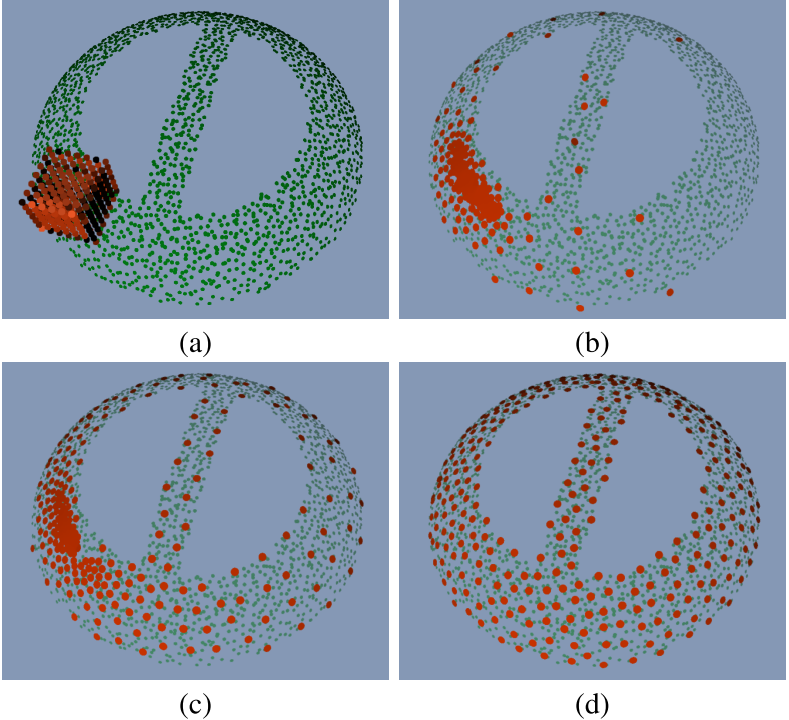
\includegraphics[width=2.0in]{images/L1median}
  \caption{Reconstruction by projection operation. (a). noisy point-set P(green) and an arbitrary point-set Q(red) that will be projected to P to approximate P. (b),(c) are two iterative projection results. (d) is the final projection.}
  \label{fig:L1 median}
\end{figure}

Reconstruction by a projection operator, as shown in Figure~\ref{fig:L1 median}, is to approximate the origin point set(green) by iteratively projecting an arbitrary point set(red) onto itself while removing the noises or outliers.
It has an important virtue: it defines a consistent geometry based on the data points, and provides constructive means to up-sample it.

$\ell_1$ median\cite{brown1983statistical,small1990survey}, closely related to projection operator, is a statistical tool applied globally to multivariate non-parametric point-samples in the presence of noises and outliers.
Briefly, it is a robust global center of an arbitrary set of points.
Given a data set $P=\{p_{j}\}_{j\in J}\subset \mathbb{R}^3$,
the $\ell_1$ median is defined as the point $q$ obtained by minimizing the sum of Euclidean distances to the data points

\small{
\begin{equation}
 \label{eq:L1median}
 q=\arg\min_{x}\left\{ \sum_{j\in J}^{}\|p_{j}-x\| \right\}
\end{equation}
}

\paragraph{(1)}

\cite{lipman2007parameterization} applies this tool locally to constitute a parameterization-free local projection operator(LOP).
Starting with an arbitrary initial point set $X^0=\{ x{_{i}^0}  \}_{i\in I}\subset \mathbb{R}^3$(typically $|X|\ll|P|$, $|\cdot|$ is the number of point set),
LOP computes the target point positions $X$ by performing a fixed-point iteration

\small{
\begin{equation}
 \label{eq:LOP1}
 X^{k+1}=\mathop{\argmin}_{X=\{x_{i}\}_{i\in I}}\{E_1(X^{k},P)+E_2(X^{k})\},\\
\end{equation}
}
\\
where,
\small{
\begin{equation}
 \label{eq:LOP2}
 \begin{split}
 & E_1(X^{k},P)=\sum_{i\in I}^{}\sum_{j\in J}^{}\|x_{i}-p_{j}\|\theta(\|x{_i^k}-p_{j}\|),\\
 & E_2(X^{k})=\sum_{i'\in I}^{}\lambda_{i'}\sum_{i\in I\setminus\{i'\}}^{} \eta(\|x_{i}-x{_{i'}^k}\|)\theta(\|x{_i^k}-x{_{i'}^k}\|).
 \end{split}
\end{equation}
}
\\
The term $E_1$ is in fact a $localized$ version of~(\ref{eq:L1median}) by using a fast-decaying weight function $\theta(r)=e^{-r^2/(h/4)^2}$ with the finite support radius $h$,
and thus it is just $E_1$ that drives the projected points $X$ to approximate the geometry of $P$.
The term $E_2$ keeps the distribution of the points $X$ fair by incorporating local repulsion forces.

To be convenient for the following works, now we give the expression of the solution. Let $\xi{_{ij}^k}=x{_i^k}-p_{j}$ and $\delta{_{ii'}^k}=x{_i^k}-x{_{i'}^k}$, solving~(\ref{eq:LOP1}), the projection for point $x{_i^{k+1}}$ is obtained as

\small{
\begin{equation}
 \label{eq:LOP3}
 x{_i^{k+1}}=F_1(x{_i^k},P)+F_2(x{_i^k},X{_i^{'}})
\end{equation}
}
\\
where,
\small{
\begin{equation}
 \label{eq:LOP4}
 \begin{split}
 & F_1(x{_i^k},P)=\sum_{j\in J}^{}p_{j}\frac{\alpha{_{ij}^k}}{\sum_{j\in J}^{}\alpha{_{ij}^k}},\\
 & F_2(x{_i^k},X{_i^{'}})=\mu\sum_{{i'}\in I\setminus\{i\}}^{}\delta{_{ii'}^k}\frac{\beta{_{ii'}^k}}{\sum_{{i'}\in I\setminus\{i\}}^{}\beta{_{ii'}^k}},\\
 & \alpha{_{ij}^k}=\frac{\theta(\|\xi{_{ij}^k}\|)}{\|\xi{_{ij}^k}\|},
   ~\beta{_{ii'}^k}=\frac{\theta(\|\delta{_{ii'}^k}\|)|\eta'(\|\delta{_{ii'}^k}\|)|}{\|\delta{_{ii'}^k}\|}.
 \end{split}
\end{equation}
}

Intuitively, LOP distributes the points by approximating their $\ell_1$ median to achieve robustness to outliers and data noises without any local orientation information nor a local manifold assumption.
But, also because of the use of the local density parameter $h$, it may not work well when the distribution of the input points is highly non-uniform and can fail to converge.

\paragraph{(2)}

Like\cite{lipman2007parameterization}, many consolidation methods try to obtain the resulted geometry object
without estimation of normals due to the unreliability resulting from the noisy data as oppose to the fact that
oriented normals at the points play a critical role in geometry reconstruction.

To achieve a better normal estimation that requires the sampling points to be uniformly distributed,
\cite{huang2009consolidation} incorporates locally adaptive density weights into LOP, resulting in a new consolidation technique WLOP, to address the non-uniform distribution problem while taking advantage of the success of LOP in denoising and outlier removal.

They define the weighted local densities for each point $p_{j}$ in $P$ and $x_{i}$ in $X$ during the $k$th iteration by $v_{j}=1+\sum_{j'\in J\setminus\{j\}}^{}\theta(\|p_{j}-p_{j'}\|)$ and $w{_i^k}=1+\sum_{i'\in I\setminus\{i\}}^{}\theta(\|\delta{_{ii'}^k}\|)$, the term $F_1$ and $F_2$ in~(\ref{eq:LOP4}) finally becomes

\small{
\begin{equation}
 \label{eq:WLOP}
 \begin{split}
 & F_1(x{_i^k},P)=\sum_{j\in J}^{}p_{j}\frac{\alpha{_{ij}^k}/v_{j}}{\sum_{j\in J}^{}(\alpha{_{ij}^k}/v_{j})}\\
 & F_2(x{_i^k},X{_i^{'}})=\mu\sum_{{i'}\in I\setminus\{i\}}^{}\delta{_{ii'}^k}\frac{w{_{i'}^k}\beta{_{ii'}^k}}{\sum_{{i'}\in I\setminus\{i\}}^{}(w{_{i'}^k}\beta{_{ii'}^k})},
 \end{split}
\end{equation}
}
\\
The weighted local density $v$ in $F_1$ relaxes the attraction of point clusters and
repulsion force in dense areas is strengthened by the local density $w$ in $F_2$.

Here, the obtained uniformly distributed point set can largely improve the reliability of normal initialization for a second normal estimation phase.
Practically, due to the high computational effort, it may not be a preferable choice to use this consolidation technique as a preprocessing method for surface reconstruction, even though some high quality surface can be reconstructed.


\paragraph{(3)}
In LOP/WLOP, the majority of the time is spent on the evaluation of the attractive forces from all points in $P$,
so \cite{preiner2014CPF} efficiently reduce the set $P$ of unordered input points to a much more compact mixture of Gaussians $\mathcal{M}=\{w_{s},\Theta_{s}\}$ that reflects the density distribution of the points.
That is, $\mathcal{M}$ defines a probability density function(pdf) as a weighted sum of $|\mathcal{M}|$ Gaussian components

\small{
\begin{equation}
 \label{eq:CLOP1}
 f(\mathbf{x}|\mathcal{M})=\sum_{s}^{}w_{s}g(\mathbf{x}|\Theta_{s}),
\end{equation}
}
\\
where the $\Theta_{s}=(\mu_{s},\sum_{s}^{})$ are the Gaussian parameters,
$w_{s}$ are their corresponding convex weights, and
$g$ denotes the $d$-variate Gaussian pdf.
%with $g(\mathbf{x}|\mu,\sum)=|2\pi\sum_{}^{}|^{-\frac{1}{2}}e^{-\frac{1}{2}(\mathbf{x}-\mu)^{T}\sum_{}^{-1}(\mathbf{x}-\mu)}$.

They define a $continuous$ $\mathcal{F}_1$ corresponding to $F_1$ in~(\ref{eq:LOP4}) by the convex sum over the internal attraction of each single Gaussian, with convex weights $w_s$ accounting for the Gaussian's relative point mass:

\small{
\begin{equation}
 \label{eq:CLOP2}
 \mathcal{F}_1(q,\mathcal{M})=\sum_{s}^{}w_s\int_{\mathbb{R}^3}^{}
 \frac{\mathbf{x}g(\mathbf{x}|\Theta_{s})\alpha(\mathbf{x})}
 {\sum_{s'}^{w_{s'}}\int_{\mathbb{R}^3}^{}g(\mathbf{x'}|\Theta_{s'})\alpha(x')d\mathbf{x}'}
 d\mathbf{x},
\end{equation}
}
\\
and the final \textbf{closed form} is expressed as
\small{
\begin{equation}
 \label{eq:CLOP3}
 \mathcal{F}_1(q,\mathcal{M})=\frac{\sum_{s}^{}\sum_{k}^{}\int_{\mathbb{R}^3}^{}\mathbf{x}\widehat{\Omega}_{sk}(\mathbf{x})d\mathbf{x}}
 {\sum_{s}^{}\sum_{k}^{}\int_{\mathbb{R}^3}^{}\widehat{\Omega}_{sk}(\mathbf{x})d\mathbf{x}}
 =\frac{\sum_{s,k}^{}w_{sk}\mu_{sk}}
 {\sum_{s,k}^{}w_{sk}}
\end{equation}
}
\\
changing the convex sum of 3D points $p_{j}$~(\ref{eq:LOP2}) into a convex combination of the product Gaussians' means $\mu_{sk}$ with weights $w_{sk}$.
Figure~\ref{fig:L1 median consolidation} shows the results of these three methods.

This continuous method is up to 7 times faster than an optimized GPU implementation of LOP/WLOP, and achieves interactive frame rates for moderately sized point clouds though it can not automatically get the best choice of the parameters for different point set.

\begin{figure}[ht]
  \centering
  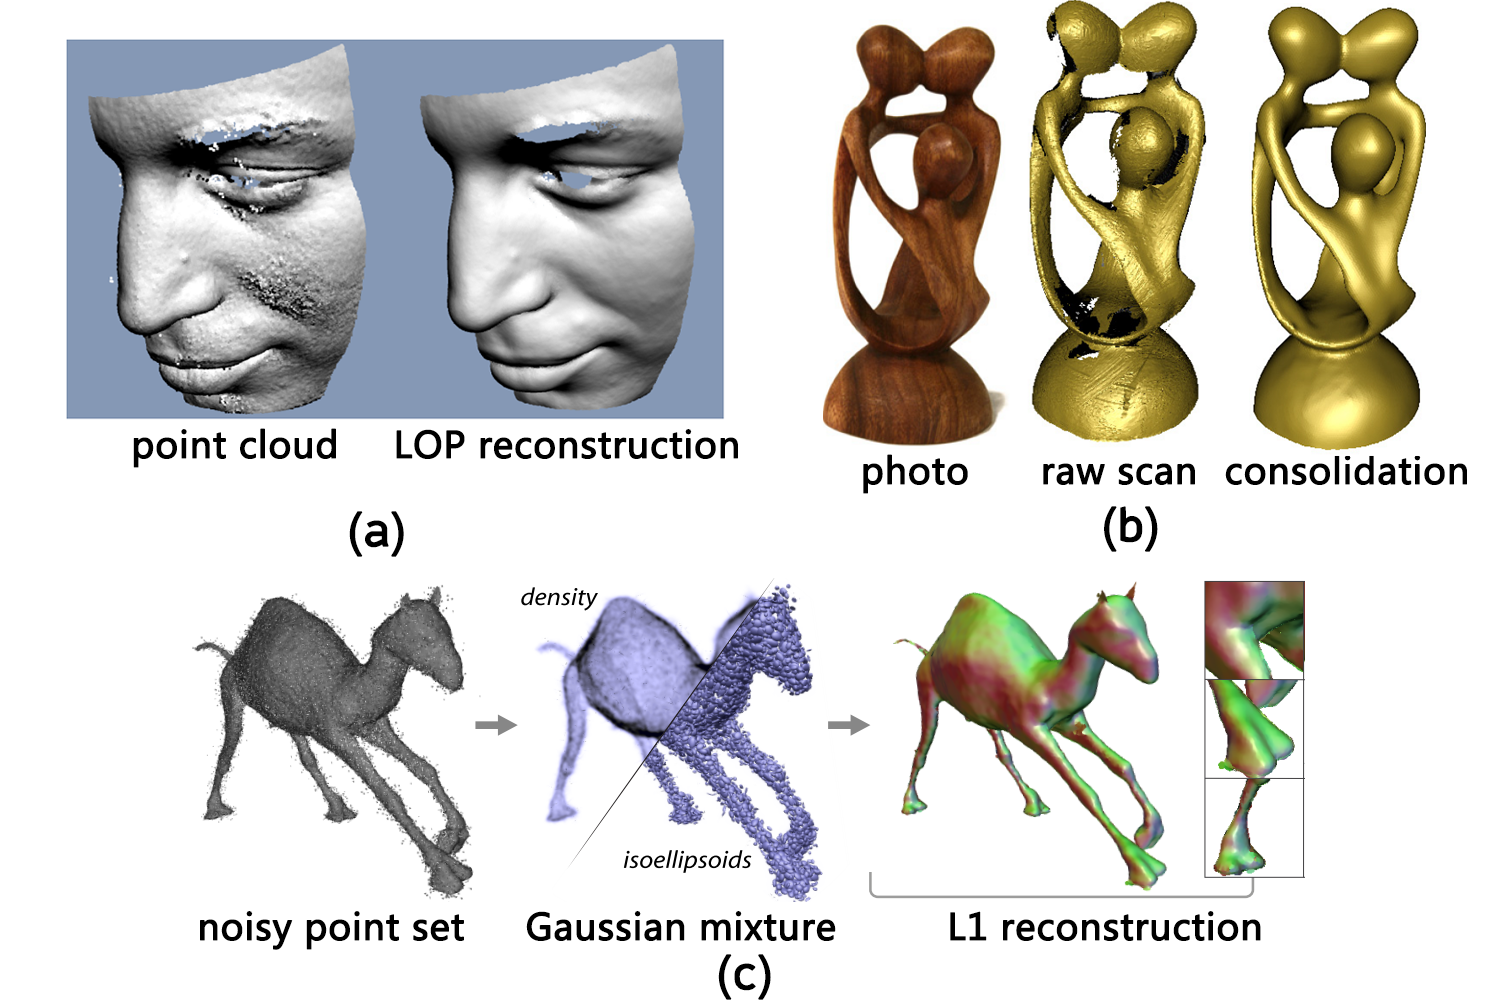
\includegraphics[width=2.5in]{images/reconstruction_L1}
  \caption{Sparse regularization: point cloud consolidation. (a): LOP\cite{lipman2007parameterization}. (b): WOLP\cite{huang2009consolidation}. (c): continuous WLOP\cite{preiner2014CPF}.}
  \label{fig:L1 median consolidation}
\end{figure}


\subsubsection{$\ell_1$ regression based}
Due to the robustness to noises and outliers of $\ell_1$ norm,
\cite{mustafa2014subdivision} develops an $\ell_1$ regression based subdivision algorithm for curve and surface fitting, 
where the size of target point cloud is largely more than that of origin data in contrast to the previous consolidation works.

For curve fitting, they try to find the best fit straight line $f(x)=\beta_1+\beta_2 x$ with observations$(x_r=r, f_r),r=-n+1,\cdots,n$.
The $\ell_1$ regression optimization is simply formulated as

\small{
\begin{equation}
 \label{eq:subdivision}
 \begin{split}
 &\beta_1, \beta_2 = \arg \min_{\beta_1,\beta_2\in\mathbb{R}}  \sum_{r=-n+1}^{n}  | f_r - (\beta_1 + \beta_2 r) |\\
 &~~~~~~~~=\arg \min_{\beta_1,\beta_2\in\mathbb{R}} F(\beta_1,\beta_2),
 \end{split}
\end{equation}
}
\\
because of the lack of differentiability, they regularize $F$ with a family of convex functional $F_{\delta}$, $\delta>0$,

\small{
\begin{equation}
 \label{eq:subdivision regularization}
 \begin{split}
 &F_{\delta}(\beta_1, \beta_2) = \sum_{r=-n+1}^{n}  h_{\delta}( f_r -\beta_1 - \beta_2 r),~\textrm{where}\\
 &h_{\delta}( f_r -\beta_1 - \beta_2 r) = [( f_r -\beta_1 - \beta_2 r)^2+\delta]^{1/2}
 \end{split}
\end{equation}
}
\\
then for a given $\delta$, the solution of (\ref{eq:subdivision}) is approximated by $\beta_{1,\delta}$ and $\beta_{2,\delta}$.
By substituting optimum $\beta_{1,\delta}$, $\beta_{2,\delta}$ into $f(x)$ and evaluating this function at 1/4 and 3/4,
the closed form of $\ell_1$ scheme for curve fitting is obtained.

With the closed form, $\ell_1$ scheme $D_{2n}$ firstly iteratively assigns weights to only $2n$ local initial points,
then gets the final fitting result(e.g.,Figure~\ref{fig:subdivision}) through subdivision rule for locations of vertices of the new mesh
and topological rule for size of added vertices and their connectivity.


\begin{figure}[ht]
  \centering
  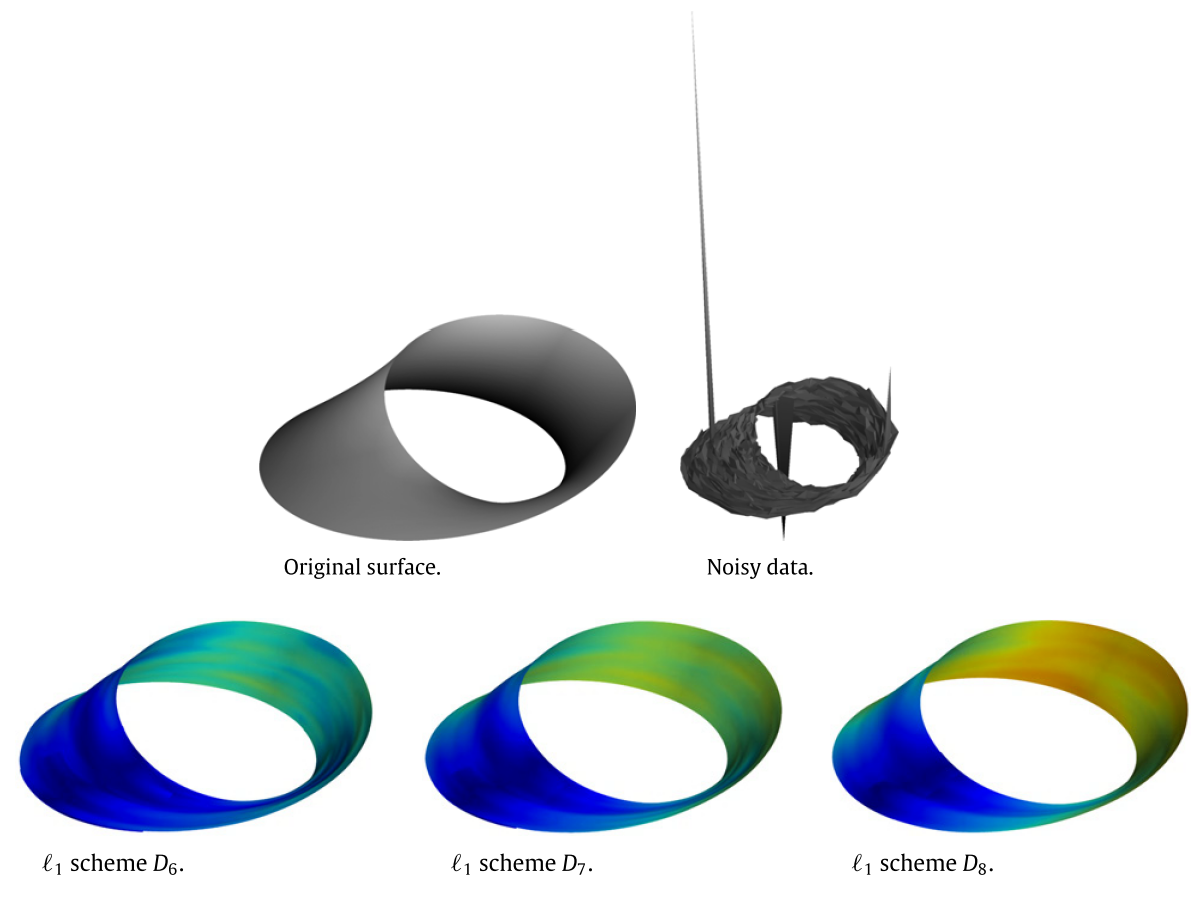
\includegraphics[width=2.5in]{images/subdivision}
  \caption{Sparse regularization: $\ell_1$ based subdivision\cite{mustafa2014subdivision}. Parametric surface reconstructed by $\ell_1$ scheme from highly noisy parametric data with outliers.}
  \label{fig:subdivision}
\end{figure}   % denoising
\subsection{Point Cloud Consolidation}
\label{subsec:Point Cloud Consolidation}


Nowadays, reconstructing the geometry of a shape from scanned data, also called point cloud consolidation, is a convenient and direct way to obtain 3D models.
It can be a preprocessing phase for some geometry problem, e.g., surface reconstruction whose result is a mesh object, with functionalities such as denoising, outlier removal, thinning, orientation, and redistribution of the input points.
However, current scanners are capable of producing large amount of raw, dense point sets with a variety of acquisition errors like noise, outliers, missing data(holes) or registration artifacts.
Then finding a robust reconstruction technique has always been an active researching area, and indeed there have been lots of works.
The works introduced in this section are all based on the $L_1$ median.

\subsubsection{$L_1$ median based}
\label{subsubsec:$L_1$ median based}

\begin{figure}[ht]
  \centering
  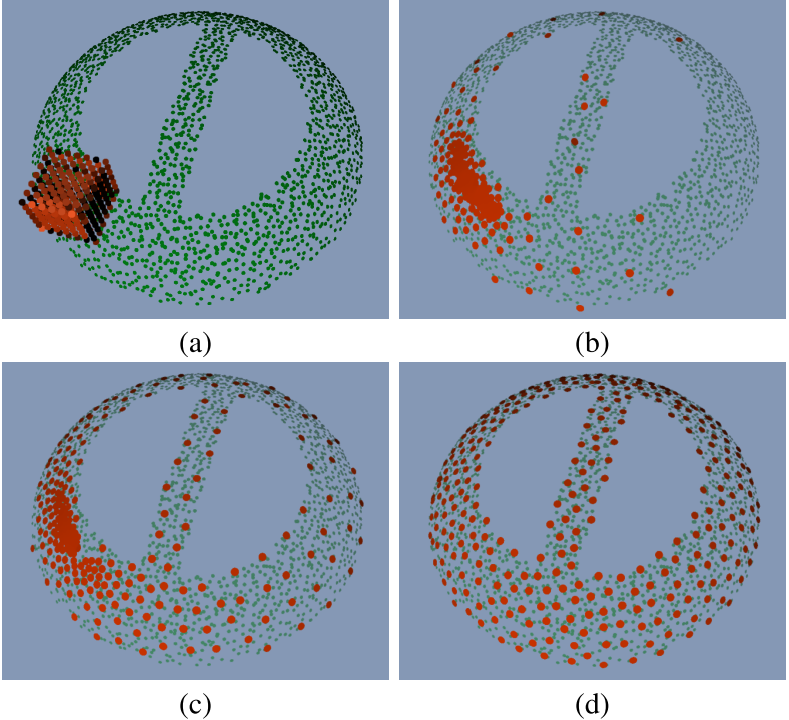
\includegraphics[width=2.5in]{images/L1median}
  \caption{Reconstruction by projection operation. (a). noisy point-set P(green) and an arbitrary point-set Q(red) that will be projected to P to approximate P. (b),(c) are two iterative projection results. (d) is the final projection.}
  \label{fig:L1 median}
\end{figure}

Reconstruction by a projection operator, as shown in Figure~\ref{fig:L1 median}, is to approximate the origin point-set(green) by iteratively projecting an arbitrary point-set(red) onto itself while removing the noises or outliers.
It has an important virtue: it defines a consistent geometry based on the data points, and provides constructive means to up-sample it.

A new projection operator is introduced via a certain fixed-point iteration where the approximated geometry consists of its stationary points,
and it is closely related to the $L_1$ median\cite{brown1983statistical,small1990survey} which is a statistical tool that applied globally to multivariate non-parametric point-samples in the presence of noise and outliers.
Briefly, it is a robust global center of an arbitrary set of points. Mathematically, given a data set $P=\{p_{j}\}_{j\in J}\subset \mathbb{R}^3$, the $L_1$ median is defined as the point $q$ obtained by minimizing the sum of Euclidean distances to the data points

\small{
\begin{equation}
 \label{eq:L1median}
 q=\arg\min_{x}\left\{ \sum_{j\in J}^{}\|p_{j}-x\| \right\}
\end{equation}
}

\paragraph{(1)}

\cite{lipman2007parameterization} applies this tool locally to constitute a robust reconstruction mechanism called parameterization-free local projection operator(LOP).
Starting with an arbitrary initial point-set $X^{(0)}=\{{x_{i}}^{(0)}\}_{i\in I}\subset \mathbb{R}^3$(typically $|X|\ll|P|$, $|\cdot|$ is the number of point-set),
LOP computes the target point positions $X$ by performing a fixed-point iteration

\small{
\begin{equation}
 \label{eq:LOP1}
 X^{k+1}=\mathop{\argmin}_{X=\{x_{i}\}_{i\in I}}\{E_1(X^{k},P)+E_2(X^{k})\},\\
\end{equation}
}
\\
where,
\small{
\begin{equation}
 \label{eq:LOP2}
 \begin{split}
 & E_1(X^{k},P)=\sum_{i\in I}^{}\sum_{j\in J}^{}\|x_{i}-p_{j}\|\theta(\|x{_i^k}-p_{j}\|),\\
 & E_2(X^{k})=\sum_{i'\in I}^{}\lambda_{i'}\sum_{i\in I\setminus\{i'\}}^{} \eta(\|x_{i}-x{_{i'}^k}\|)\theta(\|x{_i^k}-x{_{i'}^k}\|).
 \end{split}
\end{equation}
}
\\
The term $E_1$ is in fact a localized version of~(\ref{eq:L1median}) by using a fast-decaying weight function $\theta(r)=e^{-r^2/(h/4)^2}$ with the finite support radius $h$,
and thus it is just $E_1$ that drives the projected points $X$ to approximate the geometry of $P$.
The term $E_2$ keeps the distribution of the points $X$ fair by incorporating local repulsion forces.

Let $\xi{_{ij}^k}=x{_i^k}-p_{j}$ and $\delta{_{ii'}^k}=x{_i^k}-x{_{i'}^k}$, solving~(\ref{eq:LOP1}), the projection for point $x{_i^{k+1}}$ is obtained as

\small{
\begin{equation}
 \label{eq:LOP3}
 x{_i^{k+1}}=F_1(x{_i^k},P)+F_2(x{_i^k},X{_i^{'}})
\end{equation}
}
\\
where,
\small{
\begin{equation}
 \label{eq:LOP4}
 \begin{split}
 & F_1(x{_i^k},P)=\sum_{j\in J}^{}p_{j}\frac{\alpha{_{ij}^k}}{\sum_{j\in J}^{}\alpha{_{ij}^k}},\\
 & F_2(x{_i^k},X{_i^{'}})=\mu\sum_{{i'}\in I\setminus\{i\}}^{}\delta{_{ii'}^k}\frac{\beta{_{ii'}^k}}{\sum_{{i'}\in I\setminus\{i\}}^{}\beta{_{ii'}^k}},\\
 & \alpha{_{ij}^k}=\frac{\theta(\|\xi{_{ij}^k}\|)}{\|\xi{_{ij}^k}\|},
   ~\beta{_{ii'}^k}=\frac{\theta(\|\delta{_{ii'}^k}\|)|\eta'(\|\delta{_{ii'}^k}\|)|}{\|\delta{_{ii'}^k}\|}.
 \end{split}
\end{equation}
}

Intuitively, LOP distributes the points by approximating their $L_1$ median to achieve robustness to outliers and data noises without any local orientation information nor a local manifold assumption.
However, also because of the use of the local density parameter $h$, it may not work well when the distribution of the input points is highly non-uniform and can fail to converge.

\paragraph{(2)}

Like\cite{lipman2007parameterization}, many surface reconstruction methods try to obtain the resulted mesh without estimation of normals due to the unreliability because of the noisy data.
In fact, oriented normals at the points play a critical role in surface reconstruction and the estimation of normals requires the sampling points to be uniformly distributed.
\cite{huang2009consolidation} proposes a new consolidation technique whose central task is normal estimation.

To take advantage of the success of LOP in denoising and outlier removal, and simultaneously address the non-uniform distribution problem, they incorporate locally adaptive density weights into LOP, resulting in WLOP, they define the weighted local densities for each point $p_{j}$ in P and $x_{i}$ in X during the $k$th iteration by $v_{j}=1+\sum_{j'\in J\setminus\{j\}}^{}\theta(\|p_{j}-p_{j'}\|)$ and $w{_i^k}=1+\sum_{i'\in I\setminus\{i\}}^{}\theta(\|\delta{_{ii'}^k}\|)$, the term $F_1$ and $F_2$ in () finally becomes

\small{
\begin{equation}
 \label{eq:WLOP}
 \begin{split}
 & F_1(x{_i^k},P)=\sum_{j\in J}^{}p_{j}\frac{\alpha{_{ij}^k}/v_{j}}{\sum_{j\in J}^{}(\alpha{_{ij}^k}/v_{j})}\\
 & F_2(x{_i^k},X{_i^{'}})=\mu\sum_{{i'}\in I\setminus\{i\}}^{}\delta{_{ii'}^k}\frac{w{_{i'}^k}\beta{_{ii'}^k}}{\sum_{{i'}\in I\setminus\{i\}}^{}(w{_{i'}^k}\beta{_{ii'}^k})},
 \end{split}
\end{equation}
}
\\
The weighted local density $v$ in $F_1$ relaxes the attraction of point clusters and repulsion force in dense areas is strengthened by the local density $w$ in $F_2$.

So far, we actually have obtained a reconstructed point set which will then be used to improve the reliability of normal initialization that will be used in a second normal estimation phase.
However, considering the high computational effort, it may not be a preferable choice using this consolidation technique as a preprocessing method for surface reconstruction even though some high quality surface can be reconstructed.


\paragraph{(3)}
In LOP/WLOP, the majority of the time is spent on the evaluation of the attractive forces from all points in $P$,
so \cite{preiner2014CPF} efficiently reduce the set $P$ of unordered input points to a much more compact mixture of Gaussians $\mathcal{M}=\{w_{s},\Theta_{s}\}$ that reflects the density distribution of the points.
That is, $\mathcal{M}$ defines a probability density function(pdf) as a weighted sum of $|\mathcal{M}|$ Gaussian components

\small{
\begin{equation}
 \label{eq:CLOP1}
 f(\mathbf{x}|\mathcal{M})=\sum_{s}^{}w_{s}g(\mathbf{x}|\Theta_{s}),
\end{equation}
}
\\
where the $\Theta_{s}=(\mu_{s},\sum_{s}^{})$ are the Gaussian parameters, $w_{s}$ their corresponding convex weights, and $g$ denotes the $d$-variate Gaussian pdf with $g(\mathbf{x}|\mu,\sum)=|2\pi\sum_{}^{}|^{-\frac{1}{2}}e^{-\frac{1}{2}(\mathbf{x}-\mu)^{T}\sum_{}^{-1}(\mathbf{x}-\mu)}$.

They define a $continuous$ $\mathcal{F}_1$ corresponding to $F_1$ in~(\ref{eq:LOP4}) by the convex sum over the internal attraction of each single Gaussian, with convex weights $w_s$ accounting for the Gaussian's relative point mass:

\small{
\begin{equation}
 \label{eq:CLOP2}
 \mathcal{F}(q,\mathcal{M})=\sum_{s}^{}w_s\int_{\mathbb{R}^3}^{}
 \frac{\mathbf{x}g(\mathbf{x}|\Theta_{s})\alpha(\mathbf{x})}
 {\sum_{s'}^{w_{s'}}\int_{\mathbb{R}^3}^{}g(\mathbf{x'}|\Theta_{s'})\alpha(x')d\mathbf{x}'}
 d\mathbf{x},
\end{equation}
}
\\
and the final \textbf{closed form} is expressed as
\small{
\begin{equation}
 \label{eq:CLOP3}
 \mathcal{F}(q,\mathcal{M})=\frac{\sum_{s}^{}\sum_{k}^{}\int_{\mathbb{R}^3}^{}\mathbf{x}\widehat{\Omega}_{sk}(\mathbf{x})d\mathbf{x}}
 {\sum_{s}^{}\sum_{k}^{}\int_{\mathbb{R}^3}^{}\widehat{\Omega}_{sk}(\mathbf{x})d\mathbf{x}}
 =\frac{\sum_{s,k}^{}w_{sk}\mu_{sk}}
 {\sum_{s,k}^{}w_{sk}},
\end{equation}
}
\\
where in the same way that~(\ref{eq:LOP2}) is convex of 3D points $p_{j}$, now becomes a convex combination of the product Gaussians' means $\mu_{sk}$ with weights $w_{sk}$.

This method is up to 7 times faster than an optimized GPU implementation of LOP/WLOP, and achieves interactive frame rates for moderately sized point clouds though it can not automatically get the best choice of the parameters for different point set.

\vspace{10pt}
Figure~\ref{fig:L1 median consolidation} shows the results of these three methods. In summary, many robust point cloud consolidation or surface reconstruction techniques have been developed to deal with a variety of acquisition errors like noise, outliers, missing data(holes) or registration artifacts.
Most of the $l_1$ techniques are typically too expensive to achieve interactive reconstruction times for at least moderately sized point sets, even for parallel implementations,
and are designed for quality rather than performance due to their nature. So the performance problem is still challenging and worth researching. 

\begin{figure}[ht]
  \centering
  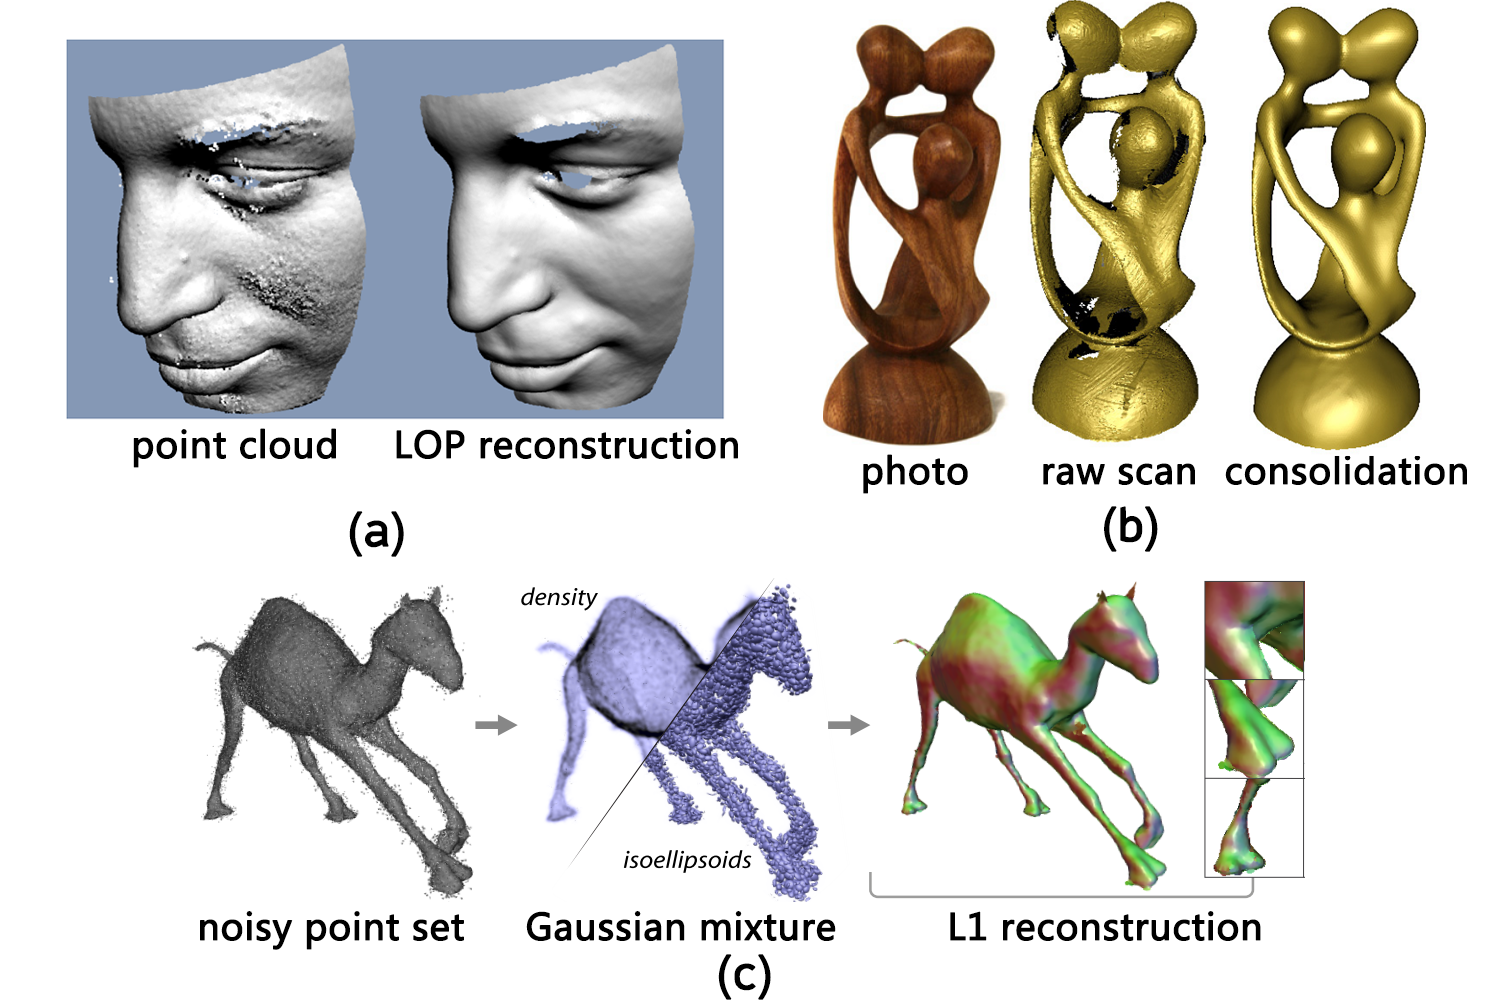
\includegraphics[width=3in]{images/reconstruction_L1}
  \caption{Sparse regularization: point cloud consolidation. (a): LOP\cite{lipman2007parameterization}. (b): WOLP\cite{huang2009consolidation}. (c): continuous WLOP\cite{preiner2014CPF}.}
  \label{fig:L1 median consolidation}
\end{figure}  % reconstruction based on L_1 median
\subsection{Shape Matching}
\label{subsec:Shape Matching}


Here, we give shape matching a more extensive definition: finding the correspondence(point-wise, pair-wise) between two rigid or non-rigid deformable geometric data sets.

\subsubsection{Rigid registration}
\label{subsubsec:Rigid registration}

Rigid registration is a fundamental task in computer graphics and geometry processing.
It aims at finding a suitable set of corresponding points on source and target point set.
The $Iterative~Closest~Point$(ICP) addresses this problem by assuming the input data to be in coarse alignment.
Under this assumption, a set of correspondences can be obtained by querying closest points on the target geometry.
Given two surfaces $\mathcal{X}$, $\mathcal{Y}$, it is formulated as

\small{
\begin{equation}
 \label{eq:ICP}
 \mathop{\argmin}_{R,t}\int_{\mathcal{X}}^{}\varphi(R\mathbf{x}+t,\mathcal{Y})d\mathbf{x}+I_{\mathcal{SO}(k)}(R)
\end{equation}
}
\\
where $R$ is a rotation matrix,
$t$ is a translation vector,
$\mathbf{x}$ is a point on the source geometry.
The quality of a registration is evaluated by the metric $\varphi(\mathbf{x},\mathbf{y})=\|\mathbf{x}-\mathbf{y}\|{_2^2}$, i.e., classical ICP is in a least-square sense which would fail with outliers.

Now that sparse regularization methods excels in processing data set with noises or outliers,
\cite{bouaziz2013sparse} tries to formulate the local alignment problem as recovering rigid transformation that minimizes the number of zero distances between two correspondences.
Since \cite{chartrand2007exact} shows that $\ell_{p}$ norms with $p<1$ outperform the $l_1$ norm in inducing sparsity and \cite{elad2010sparse} also illustrates the tendency of $\ell_{p}$($0<p<1$)norms to drive results to become sparse.
\cite{bouaziz2013sparse} adopts $l_{p}$($0\le p\le1$) norm based sparse regularizer to obtain an heuristic-free, robust rigid registration algorithm by modifying

\small{
\begin{equation}
 \label{eq:permutedsparse}
 \varphi(\mathbf{x},\mathbf{y})=\|\mathbf{x}-\mathbf{y}\|{_2^{p}}
\end{equation}
}

Figure~\ref{fig:sparseICP}is the registration results of sparse ICP under different values of $p$ among which it can be found that $0<p<1$ reduces better results,
but the value of $p$ is selected according to the experiments to offer a trade-off between performance and robustness which may make the sparse ICP unpractical.

\begin{figure}[ht]
  \centering
  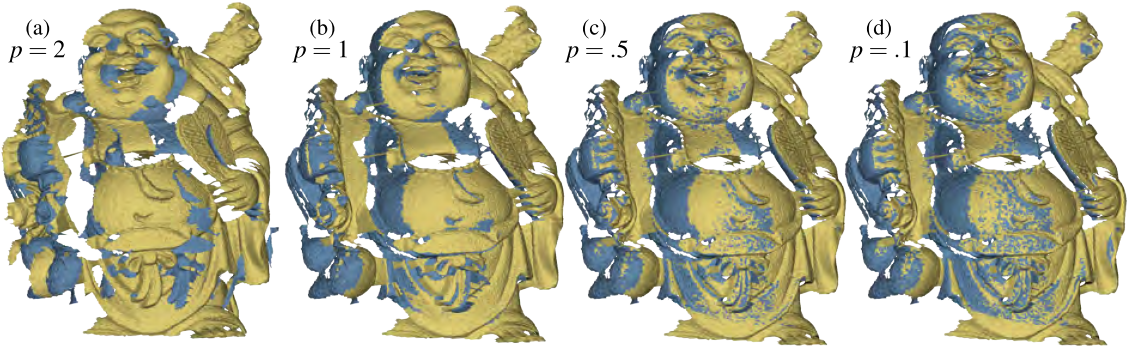
\includegraphics[width=3in]{images/sparseICP}
  \caption{Sparse regularization: rigid registration results using sparse ICP\cite{chartrand2007exact} under different $l_{p}$ norms.}
  \label{fig:sparseICP}
\end{figure}

\subsubsection{Non-rigid shape matching}
\label{subsubsec:non-rigid shape matching}

Matching of deformable shapes is a notoriously difficult problem playing an important role in many application, non-rigid matching typically uses point-wise representation of correspondence, which results in the number of degrees of freedom growing exponentially with the number of matched points.

Recently, \cite{ovsjanikov2012functional} introduces a functional representation for correspondences which are modeled as the correspondences between functions on two shapes rather than points.
Mathematically, let $X$ and $Y$ be two shapes equipped with bases $\{\phi_{i}\}_{i\ge1}$ and $\{\psi_{j}\}_{j\ge1}$ respectively,
any real function $f: X\to \mathbb{R}$ and $g=T(f): Y\to \mathbb{R}$ can be represented as $f=\sum_{i\ge1}^{}a_{i}\phi_{i}$ and $g=\sum_{j\ge1}^{}b_{j}\psi_{j}$.
Taking discretized functions $\phi_{i}$ and $\psi_{j}$ as the columns of bases matrices $\Phi$ and $\Psi$,
the function vectors can be represented as
$\mathbf{f}=\Phi \mathbf{a}$ and
$\mathbf{g}=\Psi \mathbf{b}$, and then from
$\Psi \mathbf{b}=T(\Phi \mathbf{a})=\Psi C^{T}\mathbf{a}$,
the relationship between two coefficients is clear that $\mathbf{b^{T}}=\mathbf{a^{T}}C$.
Thus, the matrix $C$ fully encodes the linear map $T$ between the functional spaces.


In case the shapes $X$ and $Y$ are isometric and the corresponding Laplace-Beltrami operators have simple spectra,
the harmonic bases(Laplacian eigenfunctions) have a compatible behavior, $\psi_{i}=T(\phi_{i})$ such that $c_{ij}=\delta_{ij}$.
Choosing the discretized eigenfunctions of the Laplace-Beltrami operator as $\Phi$ and $\Psi$ causes every low-distortion correspondence being represented by a nearly diagonal, and therefore very sparse matrix $C$.

Based on the above theory, \cite{pokrass2013sparse} firstly gets two collections of similar functions $\{f_{i}:X\to \mathbb{R}\}$ and $\{g_{j}:Y\to \mathbb{R}\}$ using some region detection process like\cite{litman2011diffusion}. \parpic[r]{\label{fig:regionmatching}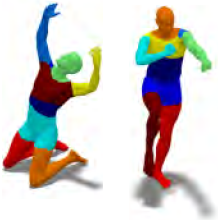
\includegraphics[width=0.4\linewidth]{images/matching_function}}As shown in the right figure, different colors represent different functions and the correspondence of these two collections of functions is unknown, i.e., we do not know to which $g_{j}$ in $Y$ a $f_{i}$ in $X$ corresponds.
\cite{pokrass2013sparse} adopts an unknown permutation matrix $\mathbf{\Pi}$ to express this ordering. Finally, the robust permuted sparse coding is formulated as following

\small{
\begin{equation}
 \label{eq:non-rigid shape matching}
 \min_{C,O,\Pi}\frac{1}{2} \|\Pi B - AC - O \|{_{F}^2} + \lambda\| W \odot C\|_1+\mu\|O\|_{2,1}
\end{equation}
}
\\
where $W$ is assigned with larger weights in off-diagonal part and small weights in diagonal part to promote diagonal solutions, $\|O\|_{2,1}$ promotes row-wise sparsity allowing to absorb the errors in the data term corresponding to the rows of $A$ having no corresponding rows in $B$.
Figure~\ref{fig:non-rigid matching} shows the correspondences between non-isometric shapes. This method relies on the region detection technique and assumption: near-isometric shapes.

\begin{figure}[ht]
  \centering
  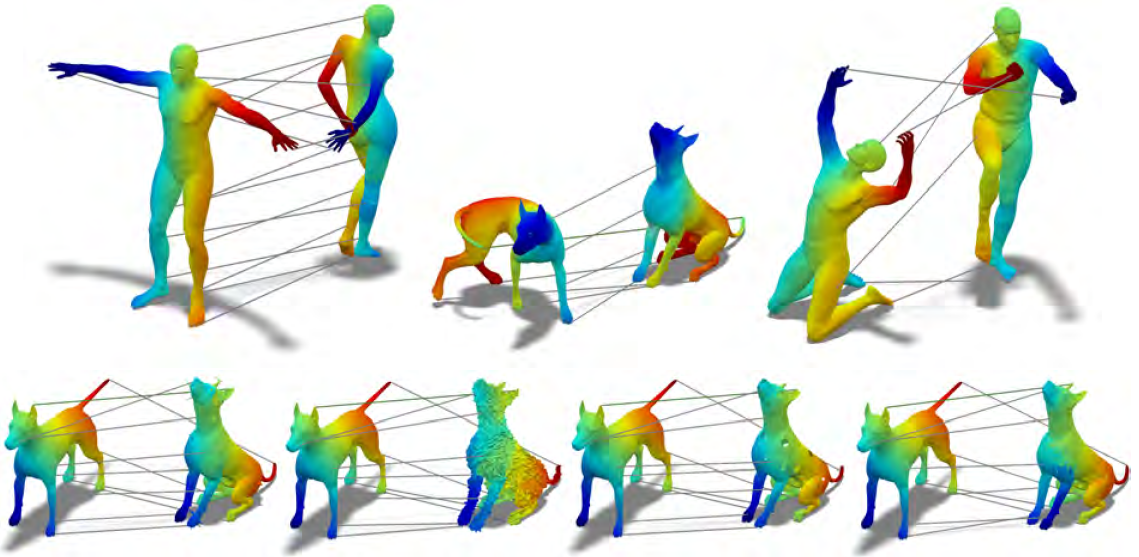
\includegraphics[width=3in]{images/matching_L1}
  \caption{Sparse regularization: non-rigid shape matching \cite{wang2014decoupling}. First row: point-to-point correspondences between different non-isometric shapes. Second row: point-to-point correspondence between SHREC shapes undergoing nearly isometric deformations and noise.}
  \label{fig:non-rigid matching}
\end{figure}


\subsubsection{Co-segmentation}
\label{subsubsec:co-segmentation}

Co-segmentation aims to consistently segment a group of shapes and obtain the correspondence between resulted segments simultaneously. As the right figure in Figure~\ref{fig:co-segmentation}shows, corresponding parts are labeled in the same colors.
To be more intuitive and efficient, \cite{hu2012co} processes co-segmentation on patch-level instead of face-level like many other works.

So they firstly over-segment all the models(left in Figure~\ref{fig:co-segmentation}) followed by calculating their feature vectors using some feature descriptors.
For example, Figure~\ref{fig:co-segmentationAGD} shows the colormaps of average geodesic distance(AGD) features of two tables with over-segmented patches, and actually there are $H=5$ feature descriptors.
They define the feature vector as a histogram of the feature measurement on the triangles of that patch.
Then it is obvious that two corresponding patches have similar distributions, which means their feature vectors lie in a common subspace generated by standard basis corresponding to these nonzero entries.
Based on this observation, they regard co-segmentation as a subspace clustering problem since the final segments are all clustering of patches.

\begin{figure}[ht]
  \centering
  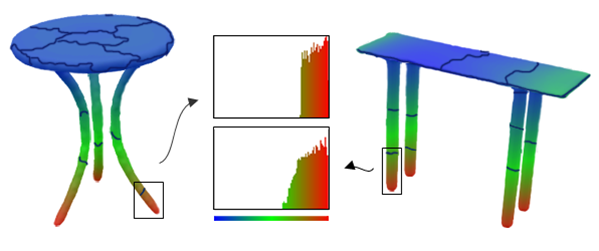
\includegraphics[width=3in]{images/co-segmentationAGD}
  \caption{Sparse regularization: co-segmentation\cite{hu2012co}. Colormaps of AGD features of two tables with over-segmented patches. The AGD feature vectors of the two patches(marked in rectangles) from each table's leg have similar distribution, as shown in histograms in the middle. It can be seen that these two feature vectors lie in the common subspace generated by standard basis corresponding to the nonzero entries.}
  \label{fig:co-segmentationAGD}
\end{figure}


Since that each data point(here is the feature vector) in a union of linear subspaces can always be represented as a linear combination of the points belonging to the same linear subspace
and thus the combination could be sparse if the point is written as a linear combination of all other points. Following\cite{elhamifar2009sparse,wang2011efficient}, finding the sparse combination matrix for the single-feature co-segmentation is formulated as

\small{
\begin{equation}
 \label{eq:SSC}
 \begin{split}
 &\min_{W_{h}}\|X_{h}W_{h}-X_{h}\|{_{F}^2}+\lambda\|W_{h}^{T}W_{h}\|_{1,1} \\
 &\mathrm{s.t.}~W_{h}\ge0,~\textrm{diag}(W_{h})=0
 \end{split}
\end{equation}
}
\\
where $h$ corresponds to the $h$-th feature descriptor,
the feature matrix $X_{h}=[x_{h1},x_{h2},\cdots,x_{hN}]$ is constructed with $x_{hi}$ which is the feature vector of the $i$-th patch($i=1,2,\cdots,N$).
$\|W_{h}^{T}W_{h}\|_{1,1}$ is seen as a penalty item in the optimization, which favors the sparsity of the optimal solution $\overline{W_{h}}$ of which each entry measures the linear correlation between two points in the meshes.
After defining the affinity matrix $S=(s_{ij})$ as $s_{ij}=|\overline{w_{h}}_{ij}|+|\overline{w_{h}}_{ji}|$, the NCut method\cite{shi2000normalized} is applied to get the co-segmentation results.

However, single one feature is not enough for co-segmenting different categories of models.
Taking two following things into account:
finding the most similar patch pairs considering selected features and corresponding patches need not be similar in these features,
\cite{hu2012co} adds the consistent multi-feature penalty to ensure the co-segmentation results consistent with different feature spaces by combing $H$ feature descriptors

\small{
\begin{equation}
 \label{eq:coseg1}
 \begin{split}
 &\min_{W_{1},\cdots,W_{H}}\sum_{h=1}^{H}\mathcal{F}(W_{h})+\mathcal{P}_{cons}(W_1,W_2,\cdots,W_H)\\
 &\mathrm{s.t.}~W_{h}\ge0,~\textrm{diag}(W_{h})=0,h=1,2,\cdots,H.
 \end{split}
\end{equation}
}
\\
where $\mathcal{P}_{cons}$ is the penalty on the matrices $W_1,W_2,\cdots,W_H$

\small{
\begin{equation}
 \label{eq:coseg2}
 \mathcal{P}_{cons}(W_1,W_2,\cdots,W_H)=\alpha\|W\|_{2,1}+\beta\|W\|_{1,1}\\
\end{equation}
}
\\
here the $H\times N^2$ matrix $W$ is formed by concatenating $W_1,W_2,\cdots,W_H$(each matrix in one row) together:

\small{
\begin{equation}
 \label{eq:coseg3}
 W = {\left[ \begin{array}{cccc}
 (W_1)_{11} & (W_1)_{12} & \cdots & (W_1)_{N^2}\\
 (W_2)_{11} & (W_2)_{12} & \cdots & (W_2)_{N^2}\\
 \vdots & \vdots & \ddots & \vdots\\
 (W_{H})_{11} & (W_{H})_{12} & \cdots & (W_{H})_{N^2}
 \end{array}
 \right]}
\end{equation}
}
\\
the $\ell_{2,1}$ penalty on $W$ induces column sparsity of $W$ such that most columns of $W$ are shrunken to be entirely zero, which means that the corresponding pairs of patches will likely not be in the same cluster.
The $\ell_{1,1}$ penalty on $W$ induces the sparsity within each column of $W$.
This means that for each non-zero column, that is for each similar patch pair, only a subset of features are actually used to measure their similarity.
Hence this term enables the prominent features to pop up and guarantees the sparsity-consistency of the matrices $W_1,W_2,\cdots,W_H$.

Notice that without $\mathcal{P}_{cons}$, the formulation~(\ref{eq:coseg1}) will reduce to a naive solution which is exactly the same as applying subspace clustering to each feature matrix $X_{h}$ independently.

\begin{figure}[ht]
  \centering
  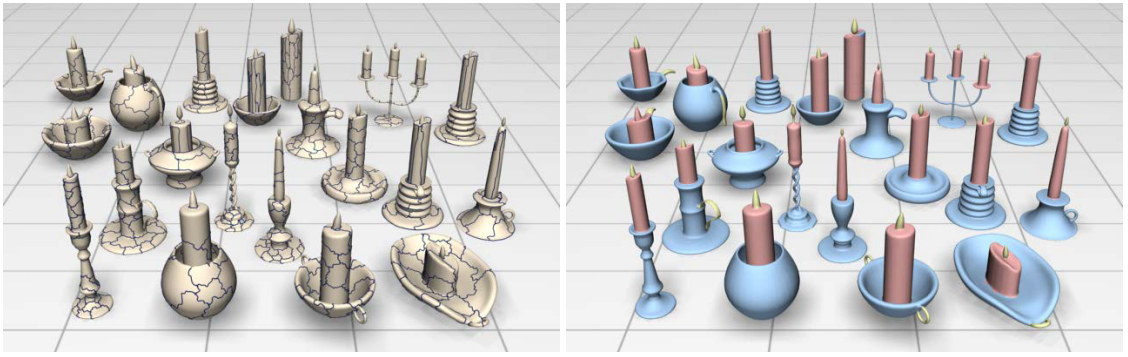
\includegraphics[width=3in]{images/co-segmentation}
  \caption{Sparse regularization: co-segmentation\cite{hu2012co}. Left shows the over segmented patches that will be clustered to get the co-segmentation result.}
  \label{fig:co-segmentation}
\end{figure}

  % shape matching



\subsection{Skeleton Extraction}
In section~\ref{subsubsec:$L_1$ median based}, we have introduced much information about $L_1$ median and its success in point cloud consolidation.
Except for reducing 2D surface that approximate origin point-set,
\cite{huang2013l1} observed that adapting $L_1$ medians $locally$ to a point set representing a geometric shape also gives rise to a $one-dimensional$ structure which can be seen as a localized center of the shape, i.e., a medial curve skeleton that can be used for shape abstraction and consequently an effective tool for shape analysis and manipulation\cite{cornea2007curve}.
Without building any point connectivity or estimating point normals, they directly project point samples onto their local centers as $l_1$ medians with growing neighborhood and push the projected samples via conditional regularization to obtain a uniform distribution of samples along skeleton branches.

It is intuitively a modification of LOP by modifying the repulsion term $E_2$ in () and proposing a different weighted density parameter that can also be named WLOP\cite{huang2009consolidation}. Re-centering. Figure~\ref{fig:skeleton extraction} shows an example.

\begin{figure}[ht]
  \centering
  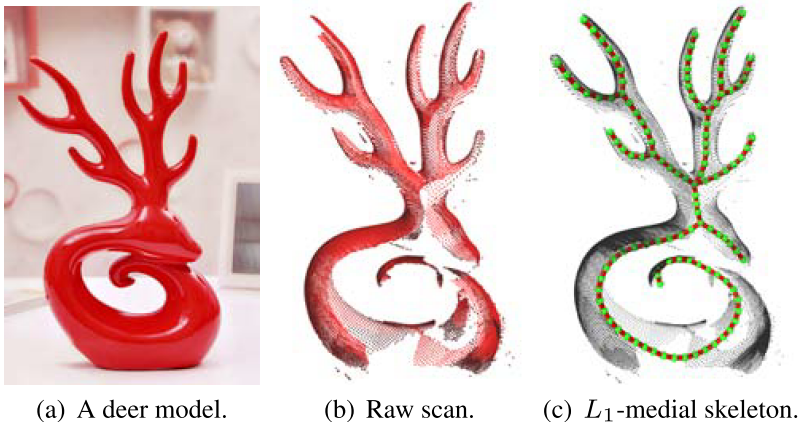
\includegraphics[width=3in]{images/skeleton_L1}
  \caption{Sparse regularization: skeleton extraction\cite{huang2013l1}. Given an unorganized, unoriented, and incomplete raw scan with noise and outliers(b), a complete and quality curve skeleton is extracted(c).}
  \label{fig:skeleton extraction}
\end{figure}


\subsection{Constrained Modeling}

Constrained modeling is an important tool for the construction and modification of 3D geometric models.
Especially in the case of modeling man-made structure like architecture or machine parts, geometric constraints are able to create and preserve ubiquitous alignment properties like element parallelism, conllinearity, fixed angles and distances, or symmetry relations.

Generally, analyzing and solving constraint systems usually fail to meet two main challenges of an interactive 3D modeling system: for each atomic editing operation,
it is crucial to adjust as few auxiliary vertices as possible in order to not destroy the user's earlier editing effort;
the whole constraint resolution pipeline is required to run in real-time to enable a fluent, interactive workflow.

To address both issues, \cite{habbecke2012linear} presents a novel interactive constrained modeling with a well-defined strategy that, for an atomic editing operation, computes $as~small~as~possible$ model updates in terms of the total number of adjusted vertices.

Mathematically, a model instance $\mathbf{X}_0$, whose elements are the vertex positions, satisfies all constraints denoted by $\mathbf{c}(\mathbf{X}_0)=\mathbf{0}$ which is a vector-valued function. Then for a given editing displacement $\mathbf{d}$ corresponding to one user editing operation, the central goal is to find a correction displacement $\mathbf{d'}$  such that $\mathbf{c}(\mathbf{X}_0+\mathbf{d}+\mathbf{d'})=\mathbf{0}$, where the zero elements of $\mathbf{d'}$ and $\mathbf{d}$ are disjoint and $\mathbf{d'}$ should be as sparse as possible.

If the space of possible movements of each vertex $\mathbf{x}_{i}$ is represented with a basis $\{\mathbf{b}_{i,1},\mathbf{b}_{i,1},\mathbf{b}_{i,3}\}$, $\mathbf{b}_{i,k} \in \mathbb{R}^3$, after extending the 3-dimensional basis vectors to vectors $\mathbf{B}_{i,k}:=(0,...,0,\mathbf{b}{_{i,k}^{T}},0,...,0) \in \mathbb{R}^{3n}$ with $3(i-1)$ leading zeros, the correction displacement $\mathbf{d'}$ can then be represented as linear combination

\small{
\begin{equation}
 \label{eq:ConstrainedModeling1}
 \mathbf{d'} := \sum_{i\notin I(\mathbf{b})}^{}\sum_{k=1}^{3}\alpha_{i,k}\mathbf{B}_{i,k}.
\end{equation}
}

So the computation of the correction of displacement $\mathbf{d'}$ is actually to compute the non-zero coefficient $\alpha_{i,k}$.
They firstly determine its non-zero set in analysis phase by solving

\small{
\begin{equation}
 \label{eq:ConstrainedModeling2}
 \sum_{i\notin I(\mathbf{d})}^{}\sum_{k=1}^{3}\alpha_{i,k}P\mathbf{B}_{i,k}=-P\mathbf{d}.
\end{equation}
}
\\
using $Orthogonal~Matching~Pursuit$(OMP)\cite{tropp2007signal},
and here $P$ is the constraints' Jacobian $J_{\mathbf{c}}\in \mathbb{R}^{m\times 3n}$.

Then the solution phase is designed to compute its values as

\small{
\begin{equation}
 \label{eq:ConstrainedModeling3}
 E(\{\alpha_{i,k}|(i,k)\in \Lambda\})=\sum_{j\in C}^{}c{_j^2}(\mathbf{X}_0+\mathbf{d}+\sum_{}^{}\alpha_{i,k}\mathbf{B}_{i,k}),
\end{equation}
}
\\
Figure~\ref{fig:constraint modeling} shows one modeling result. In this paper, each editing operation is performed on a input model instance that satisfies all predefined constraints, due to the sparsity of solutions, this strong assumption can not result in some limitations. But changing the predefined constraint types or the number of the constraints may result in failure cases.

\begin{figure}[ht]
  \centering
  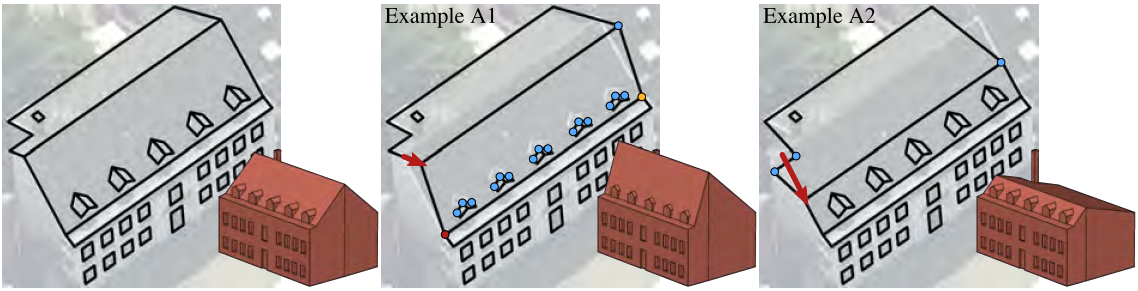
\includegraphics[width=3in]{images/modeling_L0}
  \caption{Sparse regularization: constrained modeling\cite{habbecke2012linear}. Left: original configuration. Center: editing operation such that the base plane of the dormers changes its orientation(example A1). Right: the dormers' base plane does not change(example A2). Blue vertices are relaxed in the analysis phase and automatically updated by the editing system.}
  \label{fig:constraint modeling}
\end{figure}


\subsection{Total Variation(TV) Based Applications}
\label{subsec:TV Applications}

%Total variation(TV) For a function$f(x)$ defined on a domain $\Omega\subseteq\mathbb{R}^n$, its TV is defined as
%
%\small{
%\begin{equation}
% \label{eq:continuousTV1}
% J_{f}=\int_{\Omega}^{}| \nabla f |dx,
%\end{equation}
%}
%\\
%where $| \nabla f |$ is the $\ell_2$-norm of the gradient $\nabla f$, i.e.,
%
%\small{
%\begin{equation}
% \label{eq:continuousTV2}
% | \nabla f |= \sqrt{ \sum_{i=1}^{} ( \frac{\partial f} {\partial x_{i}} )^2}.
%\end{equation}
%}
%\\

Total variation(TV) has been a popular tool for image processing tasks,such as denoising, reconstruction, and segmentation\cite{chambolle2010introduction}.
the underlying model for TV methods aims at exploiting the sparsity of the gradient of image pixel values.
The discrete variant yields the following convex objective function

\small{
\begin{equation}
 \label{eq:descreteTV}
 TV(\mathbf{u})=\sum_{i,j}^{}\|\mathcal{D}_{i,j} \mathbf{u}\|_2
\end{equation}
}
\\
where $\mathcal{D}_{i,j}$ is the discrete gradient operator at pixel $(i,j)$ and $\mathbf{u}$ is a vector containing the gray-level pixel values. TV methods filter the image by minimizing TV$(\mathbf{u})$ which is in fact the $\ell_1$ norm of the vector $[\cdots~\|\mathcal{D}_{i,j}\mathbf{u}\|_2~\cdots]$.
Since TV is designed for images, it is not directly applicable to geometry processing problem.
As we have stated, the key point is to find some form of second order information.

Note that some of the following applications have been reviewed in previous sections, but considering the good development of TV in geometry processing, we take one subsection to introduce its applications attempting to help readers understands it better.

\subsubsection{Point cloud consolidation}
\label{subsubsec:TVPoint cloud consolidation}

In section~\ref{subsec:Point Cloud Consolidation}, the consolidation works are all $\ell_1$ median based.
Here we review one more well-known work.
Similar to the sparse gradient minimization, and based on the observation that the gradients(normal differences) of smooth surface normals(normal differences) are sparse,
\cite{avron2010L1} formulates the piecewise smoothness reconstruction problem as a sparse minimization of orientation differences and position projections as following

\small{
\begin{equation}
 \label{eq:TVconsolidation1}
 \begin{aligned}
 &N^{out} =\mathop{\argmin}_{N} \sum_{(p_{i},p_{j})\in E}^{} w_{i,j}\|n_{i}-n_{j}\|_2\\
 &\mathrm{s.t.}~\forall i~\|n_{i}-{n_{i}}^{in}\|_2\le \gamma_{n}
 \end{aligned}
\end{equation}
}
\small{
\begin{equation}
 \label{eq:TVconsolidation2}
 X^{out} = \mathop{\argmin}_{X} \sum_{(p_{i},p_{j})\in E}^{} w_{i,j}|n_{i,j}\cdot (x_{i}-x_{j})|
\end{equation}
}
\\
where $\{n_{i}\}$ denote the surface normals, $\{x_{i}\}$ denote the point positions and $\{w_{i,j}\}$ is a set of the weight whose role is to achieve lower-than-$\ell_1$ sparsity.

Convexity of these two problems allows for finding a global optimum and deriving efficient solvers.
Figure~\ref{fig:TV consolidation} shows a well reconstructed example with sharp features.
Due to the global nature, this algorithm is extremely slow.
And it may fail for the point set with severe noises and outliers.

\begin{figure}[ht]
  \centering
  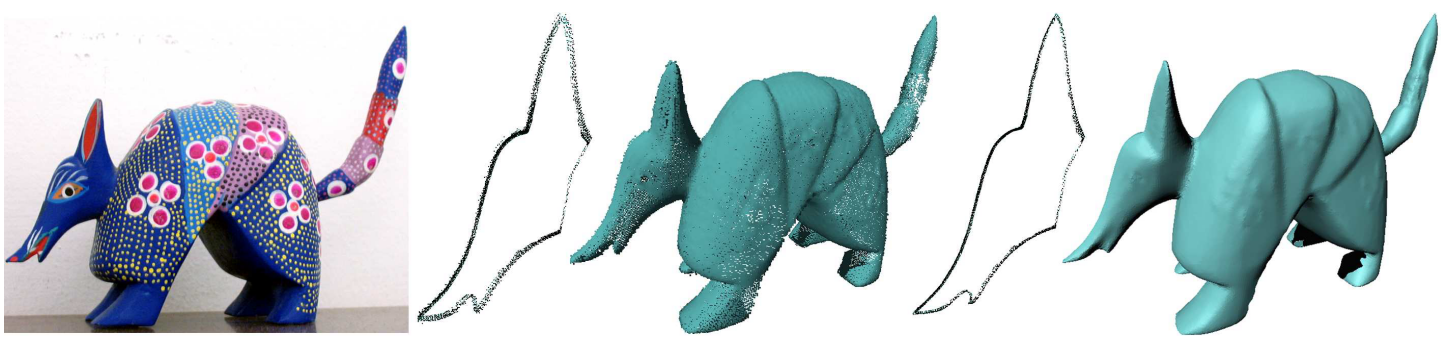
\includegraphics[width=3in]{images/TV_consolidation}
  \caption{Sparse regularization: TV based point cloud consolidation\cite{lipman2007parameterization}. The Armadillo statue(left) is scanned generating a noisy point-cloud(middle). The right figure shows the consolidation result preserving the sharp features.}
  \label{fig:TV consolidation}
\end{figure}


\subsubsection{Mesh Denoising}
\label{subsubsec:mesh denoising}
Unlike\cite{he2013mesh} achieving denoising with a new proposed edge operator, \cite{zhang2014variational}, adopting the sparsity of face normals differences, proposes a two-phase method including $face$ normal filtering and vertex updating.
They filter face normals with a new variational denoising method based on the definition of piecewise constant function spaces and associated differential operators on triangulated surfaces.

\paragraph{Piecewise constant function spaces and operators}
For a space $V_{M}=\mathbb{R}^{T}$ equipped with well-defined inner product and norm, it is isomorphic to the piecewise constant function space over surface $M$, i.e., $u=(u_0,u_1,\cdots, u_{T-1})\in V_{M}$, $T$ is the triangle number in $M$ and $u_{\tau}$ denotes the value of $u$ restricted on the triangle $\tau$. After defining the jump of $u\in V_{M}$ over an edge $e$ as

\small{
\begin{equation}
 \label{eq:edgejump}
 [u]_{e} := \left \{
 \begin{aligned}
 & \sum_{e\prec\tau}^{} u|_{\tau} \textrm{sgn}(e, \tau),  &e\nsubseteq \partial M \\
 & 0,  &e\subseteq \partial M
 \end{aligned}
 \right.
\end{equation}
}
\\
the gradient operator is defined as
\small{
\begin{equation}
 \label{eq:edgegradient}
 \nabla:u\rightarrow \nabla u, \nabla u|_{e}=[u]_{e},~\forall e, ~\textrm{for}~u\in V_{M}.
\end{equation}
}
\\
here, $e\prec\tau$ indicates that $e$ is an edge of the triangle $\tau$, then if the orientation of $e$ is consistent with the orientation of $\tau$, $\textrm{sgn}(e, \tau)=1$; otherwise $\textrm{sgn}(e, \tau)$=-1.

Due to the ambiguity of the tangent space at an edge, they define another space $Q_{M}=\textrm{Range}(\nabla)$. The divergence operator, div: $Q_{M}\rightarrow V_{M}$, as the adjoint operator of $-\nabla$, is formulated as

\small{
\begin{equation}
 \label{eq:edgedivergence}
 (\textrm{div}p|_{\tau})=\frac{-1}{s_{\tau}}
 \sum_{e\prec\tau,e\nsubseteq \partial M}^{}
 l_{e} p|_{e} \textrm{sgn}(e, \tau),~\forall p\in Q_{M}.
\end{equation}
}
\\
where, $s_{\tau}$ is the area of triangle $\tau$, $l_{e}$ is the length of edge $e$.
Thus for $u\in V_{M}$, the total variation is

\small{
\begin{equation}
 \label{eq:elementtv}
 R_{\textrm{tv}}(\nabla u) = (\textrm{TV})(u)
 = \sum_{e}^{} l_{e} | (\nabla u)|_{e} |
 = \sum_{e}^{} l_{e} | [u]_{e} |.
\end{equation}
}
\\
here, $l_{e}$ just meets the perimeter formulae defined using total variation of the characteristic function. To be more suitable to practical applications, they extend the above definition to vectorial case, for $_{\mathfrak{N}}$-channel data

\small{
\begin{equation}
 \label{eq:vectorialspace}
 \mathbf{V}_{M} = \underbrace{V_{M}\times\cdots\times V_{M}}_{\mathfrak{N}},
 \mathbf{Q}_{M} = \underbrace{Q_{M}\times\cdots\times Q_{M}}_{\mathfrak{N}}
\end{equation}
}
\\
and the vectorial total variation of $\mathbf{u}\in\mathbf{V}_M$ is

\small{
\begin{equation}
 \label{eq:vectorialtv}
  R_{\textrm{vtv}}(\nabla \mathbf{u}) = (\textrm{TV})(\mathbf{u})
 = \sum_{e}^{}   \sqrt{\sum_{i=1}^{\mathfrak{N}}  l_{e} | [u_{i}]|_{e} |^2} .
\end{equation}
}

\paragraph{Variational model}
Based on these definitions, they give a new variational face normals($\mathbf{N}$) filtering method formulated as

\small{
\begin{equation}
 \label{eq:denoisingmodeltv1}
 \min_{\mathbf{N}\in C_{\mathbf{N}}}
 \left\{
 R_{\textrm{wvtv}}(\nabla \mathbf{N})+
 \frac{\alpha}{2} \| \mathbf{N}-\mathbf{N}^{in} \|{_{\mathbf{V}_M}^{2}}
 \right\},
\end{equation}
}
\\
where
\small{
\begin{equation}
 \label{eq:denoisingmodeltv2}
 \begin{aligned}
 & R_{\textrm{wvtv}}(\nabla \mathbf{N})
 = \sum_{e}^{} w_{e}   \sqrt{\sum_{i=1}^{3}  l_{e} | [N_{i}]|_{e} |^2},\\
 & C_{\mathbf{N}}=\left\{ \mathbf{N}\in\mathbf{V}_M: \| \mathbf{N}_{\tau} \|_2=1,~\forall\tau  \right\}
 \end{aligned}
\end{equation}
}
\\
with $w_{e}$ as a weight aiming for improving preserving sharp features.
Iteratively solving this variational model~(\ref{eq:denoisingmodeltv1}) and updating vertex using previous method, the denoising results preserving sharp features can be obtained as shown in Figure~\ref{fig:denoise_tv}.
Like many other optimization problem, the optimal values of the parameters, like $\alpha$, are given by the experimental data and there is of course no theoretical convergence guarantee.

\begin{figure}[ht]
  \centering
  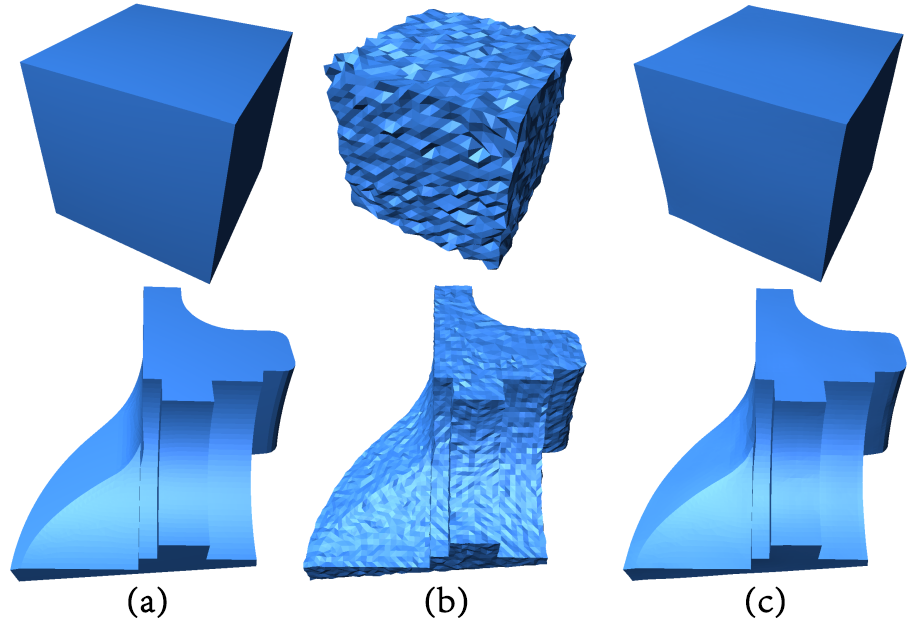
\includegraphics[width=2.5in]{images/denoise_tv}
  \caption{Sparse regularization: TV based mesh denoising\cite{zhang2014variational}. (a): clean meshes. (b): noisy mesh(Gaussian noise, standard deviation=0.2 mean edge length for Cube; standard deviation=0.1 mean edge length for Fandisk). (c): denoising result.}
  \label{fig:denoise_tv}
\end{figure}


\subsubsection{Decomposition}
\label{subsubsection:Decompsition}

Mesh decomposition means segmenting a mesh into meaningful parts that are consistent with user intention, geometric mesh attributes, and human shape perception.
Generally, the elements within the same segment should have high similarity, the segment boundary should be tight and smooth as well as matching human perception, and obviously the segmentation should reflect significant features.

Motivated by the preceding observation, \cite{zhang2012variational} proposes a new method based on the Mumford-Shah model(M-S model)\cite{mumford1989optimal} that has proven successful in image segmentation, i.e., this method is also an extension from 2D images to 3D meshes.

In 2D image $I:\Omega\rightarrow \mathbb{R}^2$, the Mumford-Shah image segmentation is to find a partition $\Omega=\bigcup{_{i=1}^{k}}\Omega_{i}$, where $\Omega_{i}$ are pairwise disjoint, and numbers $c_{i}$ for $\Omega_{i}$ formulated as

\small{
\begin{equation}
 \label{eq:TV image M-S}
 \inf_{\Omega_{i},c_{i}} \sum_{}^{k}
 ( \int_{\Omega_{i}}^{} (I(x)-c_{i})^2dx + \frac{\mu}{2} | \partial\Omega_{i} | ),
\end{equation}
}
\\
where $\mu$ is a constant, $\partial \Omega$ and $|\partial \Omega|$ represent the boundary and the boundary length of segment $\Omega$, respectively.
The first data term measures the consistency of each segment and the second regularization term measures the boundary length.

To segment a 3D triangulated surface $M$, \cite{zhang2012variational} convexifies this difficult nonconvex problem~(\ref{eq:TV image M-S}) based on TV to get a new version of M-S model

\small{
\begin{equation}
 \label{eq:TV surface M-S}
 \min_{\mathbf{u}\in K, \chi_{i}} \left \{
 \int_{M}\langle\mathbf{u}(x), \mathbf{s}(x)\rangle +
 \mu g(x)| \nabla_{M}\mathbf{u}(x) | d\sigma
 \right\},
\end{equation}
}
\\
where $K$ is the set of vector functions $\mathbf{u}=(u_1,\cdots,u_{k})^{T}:M\rightarrow \mathbb{R}^{k}$ satisfying that for all $x\in M$ and $i\in [1,\cdots,k],u_{i}(x)\geq0$ and
$\sum_{i=1}^{k}u_{i}(x)=1; \mathbf{s}(x)=(s_1(x),\cdots,s_k(x))^T$ is a $k$-dimensional vector with $s_i(x)=(\mathbf{f}(x)-\chi_{i})^{T}(\mathbf{f}(x)-\chi_{i})$ indicating
the affinity vector $\chi_{i}$ that is associated with $M_{i}$ which is a segment.
The $\mathbf{f}(x)$ is constructed with the eigenvectors of the Laplacian matrix of the dual graph of $M$ to represent some attributions of $x$ over mesh $M$ similar to the RGB function for an image.
Since the regularization term is to constrain the boundary with some geometric difference information between segments, this optimization may fail for the relative smooth models.

In~(\ref{eq:TV surface M-S}), if the affinity of $x$ with segment $M_{i}$ is large, $u_{i}(x)$ will tend to be small in order to reach the minimization,
thus $u_{i}(x)$ can be viewed as the probability of $x$ being assigned to segment $M_{i}$ and
so $\mathbf{u}(x)$ is used as a classification function for the segmentation achieved with some following processing work.
Different kind of segmentation results are shown in Figure~\ref{fig:segmentation}.


\begin{figure}[ht]
  \centering
  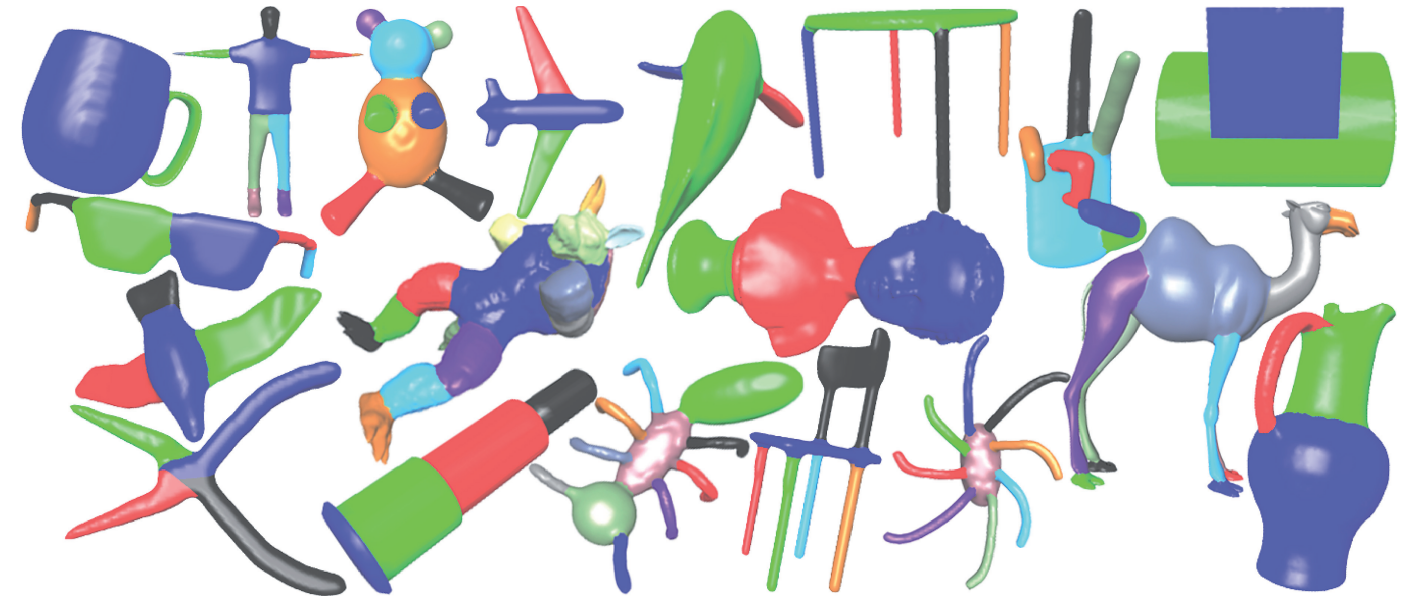
\includegraphics[width=3in]{images/segmentation}
  \caption{Sparse regularization: TV based mesh decomposition\cite{zhang2012variational}. Decomposition results where the models are taken from the Princeton Segmentation Benchmark\cite{chen2009benchmark}. One mesh is shown for each category. The segmentation results match results match human perception well in not only the cutting boundaries but also the number of segments.}
  \label{fig:segmentation}
\end{figure}


\subsubsection{Barycentric coordinates}
\label{subsubsec:Barycentric coordinates}

Barycentric~coordinates provide a simple and convenient way of interpolating values from a set of control points over the interior of a domain, using weighted combinations of values associated with different control points.
Many barycentric coordinates typically get a interpolated value depends on many, potentially $all$, control points.
Then locality, scalability, and moderate computation cost can not be achieved.

\cite{zhang2014local} introduces a novel method to derive $local~barycentric~coordinates$(LBC) that depend only on a small number of control points.
Given a set of control points $\mathbf{c}_1, \cdots, \mathbf{c}_n$ in $\mathbb{R}^2$ or  $\mathbb{R}^3$ which are the vertices of a closed control cage that bounds a domain.
The goal is to find a function $w_{i}$: $\Omega\rightarrow\mathbb{R}$ for each $\mathbf{c}_{i}$, such that $[w_1(\mathbf{x}), \cdots, w_n(\mathbf{x})]$ is a set of generalized barycentric coordinates of $\mathbf{x}\in\Omega$ with respect to the control points $\{\mathbf{c}_{i}\}$ and is used for interpolating function values $f(\mathbf{c}_1), \cdots, f(\mathbf{c}_n)$ at control points on the interior of $\Omega$ by

\small{
\begin{equation}
 \label{eq:BC}
 f(\mathbf{x}) = \sum_{i=1}^{n}w_{i}(\mathbf{x})f(\mathbf{c}_{i}),
\end{equation}
}
\\
except for the properties satisfied in many barycentric coordinate schemes, like reproduction and partition of unity,
they prefer a target $convex$ functional that also reflects $locality$ and $smoothness$ for the coordinate functions.

For a function $w_{i}$ and a given value $s$, denote by $\{w_{i}>s\}:=\{\mathbf{x}|w_{i}(\mathbf{x})>s\}$ and $\{w_{i}=s\}:=\{\mathbf{x}|w_{i}(\mathbf{x})=s\}$ the $superlevel~set$ and the $level set$ of $s$, respectively.
Locality requires the area of the superlevel set $\{w_{i}>0\}$ to be small which means that the vector$[w_{1}(\mathbf{x}), \cdots, w_{n}(\mathbf{x})]$ is sparse, while for smoothness it is necessary that all curves/surfaces $w_{i}=\textrm{const}$ are smooth.

Then the locality and smoothness of $w_{i}$ can be obtained using a functional that measures the sum of the perimeters of superlevel sets $\{w_{i}>s\}$ for all $s$.
That is, the perimeter of each superlevel set regularizes the smoothness of its boundary level curve/surface, while the perimeter of $\{w_{i}>0\}$ penalizes the area of the influence region. 
This functional is exactly the total variation of $\{w_{i}\}$ formulated as

\small{
\begin{equation}
 \label{eq:continuousLBC}
 \begin{aligned}
 & \min_{w_1, \cdots, w_2} \sum_{i=1}^{n} \int_{\Omega}^{} |\bigtriangledown w_{i}| \\
 & ~~~\mathrm{s.t.}~ \sum_{i=1}^{n}w_{i}(\mathbf{x})\mathbf{c}_{i}=\mathbf{x},
        \sum_{i=1}^{n}w_{i}=1,~w_{i}\geq0,~\forall \mathbf{x}\in\Omega,\\
 & ~~~~~~~~w_{i}(\mathbf{c}_{j})=\delta_{ij},~forall i,j,\\
 & ~~~~~~~~w_{i}~\textrm{is linear on cage edges and faces }\forall i.
 \end{aligned}
\end{equation}
}
\\
Discretely, after triangulating the domain $\Omega$, each $w_{i}$ is represented a function that is linear within each cell(triangle in 2D or tetrahedron in 3D) and then the gradient of $w_{i}$ is constant on each cell. Let $\mathcal{C}$ be the set of cells in the triangulation, the target functional~(\ref{eq:continuousLBC}) finally becomes

\small{
\begin{equation}
 \label{eq:discreteLBC}
 \sum_{T\in\mathcal{C}}^{}  \sum_{i=1}^{}
 \phi{_{i}^{T}}  A_{T}  \| \nabla T w_{i} \|_2,
\end{equation}
}
\\
where $\nabla T w_{i}$ is the gradient of $w_{i}$ in cell $T$, $A_{T}$ is the area(volume) of $T$, and $\phi{_{i}^{T}}$ is the value of the weighting function $\phi_{i}$ at the centroid of $T$.

Figure~\ref{fig:LBC} shows a cage-based deformation example with lower computational and storage requirement since each point on the target shape is only determined by a small number of control points.
Whatever, from the observation, we can see that there is a trade-off between locality and smoothness which is a common troubling issue for so many existing works.

\begin{figure}[ht]
  \centering
  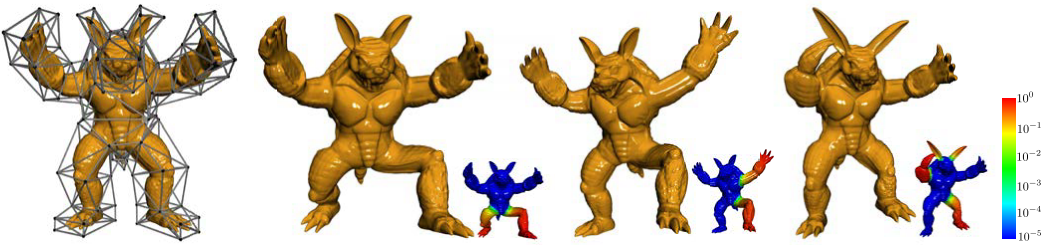
\includegraphics[width=3in]{images/LBC_L1}
  \caption{Sparse regularization: TV based local barycentric coordinates\cite{zhang2014local}. Using LBC for 3D cage-based manipulation allows for local, smooth and shape-aware deformations. Only parts near the manipulated control points are deformed, as indicated by the color-coding.}
  \label{fig:LBC}
\end{figure}
  % shape matching 